\chapter{Modeling Methodology and Results}

This chapter presents the implementation and evaluation of ensemble machine learning models for bankruptcy prediction. Two prominent ensemble methods (Bagging and Boosting style), Random Forest and XGBoost, were applied to both full and selected feature datasets, resulting in four distinct modeling approaches for comprehensive performance comparison.

Random Forest represents a robust ensemble method that combines multiple decision trees through bootstrap aggregating (bagging). Each tree in the forest is trained on a different bootstrap sample of the data, and predictions are made through majority voting for classification tasks. The method incorporates randomness at both the observation level (through bootstrap sampling) and feature level (through random feature selection at each split), reducing overfitting and improving generalization performance.
Key advantages of Random Forest for bankruptcy prediction include its ability to handle mixed data types, resistance to overfitting, implicit feature selection capabilities, and provision of feature importance measures. The method's ensemble nature makes it particularly suitable for financial data where relationships may be complex and non-linear.

XGBoost (Extreme Gradient Boosting) on the other hand, represents an advanced implementation of gradient boosting that sequentially builds decision trees to correct errors from previous iterations. Unlike Random Forest's parallel tree construction, XGBoost employs a sequential approach where each tree learns from the residuals of its predecessors, resulting in progressively improved predictions.
XGBoost incorporates several sophisticated features including regularization terms to prevent overfitting, advanced tree pruning algorithms, and optimized computational efficiency. These characteristics make it particularly effective for complex financial prediction tasks where subtle patterns and feature interactions are crucial for accurate classification.

Four distinct models were developed to enable comprehensive performance assessment:

\begin{enumerate}
    \item Random Forest with Full Features (RF\_Full): Utilizing all 63 features after X37 removal
    \item Random Forest with Selected Features (RF\_Selected): Utilizing the 15 clustered features
    \item XGBoost with Full Features (XGB\_Full): Utilizing all 63 features after X37 removal
    \item XGBoost with Selected Features (XGB\_Selected): Utilizing the 15 clustered features
\end{enumerate}

Each model employed an 80-20 train-test split with consistent random state (123) to ensure reproducible results and fair comparison across modeling approaches.

\section*{Hyperparameter Optimization}

\subsection*{Random Forest Hyperparameter Tuning}

Comprehensive hyperparameter optimization was conducted using 5-fold cross-validation with GridSearchCV. The parameter search space included:

\begin{itemize}
    \item Criterion: ['gini', 'entropy']
    \item Max features: [5, 10, 15, 20]
    \item Max depth: [None, 1, 3, 5, 7, 9]
    \item Min samples split: [8, 6, 4]
    \item Min samples leaf: [4, 2, 1]
\end{itemize}

Detailed results from hyperparameter tuning for Random Forest models are shown in Table \ref{tab:rf_hyperparams}.

\begin{table}[H]
    \centering
    \caption{Optimal Hyperparameters for Random Forest Models}
    \label{tab:rf_hyperparams}
    \begin{tabular}{lcc}
    \toprule
    \textbf{Hyperparameter} & \textbf{RF\_Full} & \textbf{RF\_Selected} \\
    \midrule
    Criterion & entropy & entropy \\
    Max Depth & None & 7 \\
    Max Features & 20 & 10 \\
    Min Samples Leaf & 2 & 2 \\
    Min Samples Split & 8 & 8 \\
    CV Score & 0.9582 & 0.9514 \\
    \bottomrule
    \end{tabular}
\end{table}

\subsection*{XGBoost Hyperparameter Tuning}

XGBoost hyperparameter optimization employed a custom random search approach with 30 iterations, optimizing AUC scores through 5-fold cross-validation. The search space included:

\begin{itemize}
    \item Max depth: [2, 4, 6, 8, 10, 12, 15, 20]
    \item Subsample: [0.5, 1.0]
    \item Colsample bytree: [0.5, 1.0]
    \item Colsample bylevel: [0.5, 1.0]
    \item Colsample bynode: [0.5, 1.0]
\end{itemize}

The optimization process identified optimal configurations for both full and selected feature models, with the full feature model achieving superior cross-validation AUC scores compared to the selected feature variant.
Detailed results from hyperparameter tuning for XGBoost models are shown in Table \ref{tab:xgb_hyperparams}.

\begin{table}[H]
    \centering
    \caption{XGBoost Hyperparameter Search Results}
    \label{tab:xgb_hyperparams}
    \begin{tabular}{lcc}
    \toprule
    \textbf{Parameter} & \textbf{Search Range} & \textbf{Optimal Configuration} \\
    \midrule
    Max Depth & [2, 4, 6, 8, 10, 12, 15, 20] & 15 (Full), 8 (Selected) \\
    Subsample & [0.5, 1.0] & 0.75 \\
    Colsample Bytree & [0.5, 1.0] & 0.8-0.9 \\
    Colsample Bylevel & [0.5, 1.0] & 0.6-0.8 \\
    Colsample Bynode & [0.5, 1.0] & 0.7-0.9 \\
    Learning Rate & Fixed & 0.1 \\
    N Estimators & Fixed & 100 \\
    \bottomrule
    \end{tabular}
\end{table}

\section*{Model Performance Results}

The performance results for all four models are shown in Table \ref{tab:model_performance}.
We can see that XGBoost models generally perform slightly better than Random Forest models, with XGBoost\_Full achieving the highest overall accuracy (96.9\%) and XGBoost\_Selected achieving the highest bankruptcy precision (0.89).
With the selected feature models, the performance is slightly lower than the full feature models, but the difference is not significant. 
The reason is that the selected feature models are not able to capture the same level of information as the full feature models.
Both Random Forest and XGBoost models are rooted in tree-based model, which does not require feature scaling. Therefore, it is not necessary to scale the features for these models as shown in the EDA section.

\begin{table}[H]
    \centering
    \caption{Comprehensive Model Performance Comparison}
    \label{tab:model_performance}
    \begin{tabular}{lcccc}
    \toprule
    \textbf{Metric} & \textbf{RF\_Full} & \textbf{RF\_Selected} & \textbf{XGB\_Full} & \textbf{XGB\_Selected} \\
    \midrule
    \textbf{Overall Accuracy} & 95.5\% & 94.8\% & 96.9\% & 94.9\% \\
    \textbf{Bankruptcy Precision} & 0.56 & 0.05 & 0.89 & 0.17 \\
    \textbf{Bankruptcy Recall} & 0.07 & 0.01 & 0.36 & 0.03 \\
    \textbf{Bankruptcy F1-score} & 0.12 & 0.01 & 0.52 & 0.05 \\
    \textbf{Macro Avg F1-score} & 0.55 & 0.49 & 0.75 & 0.51 \\
    \textbf{Weighted Avg F1-score} & 0.94 & 0.93 & 0.96 & 0.93 \\
    \bottomrule
    \end{tabular}
\end{table}

Receiver Operating Characteristic (ROC) analysis serves as the primary evaluation framework for assessing model discriminative ability across all decision thresholds. ROC curves plot the True Positive Rate (Sensitivity) against the False Positive Rate (1-Specificity), providing a threshold-independent assessment of classification performance. The Area Under the Curve (AUC) summarizes this performance into a single metric, where values closer to 1.0 indicate superior discriminative ability.

The ROC analysis revealed substantial performance differences across the four modeling approaches. Figure \ref{fig:roc_curves} presents the complete ROC curves for all models, demonstrating clear performance hierarchies and the impact of both algorithmic choice and feature selection strategies.

\begin{figure}[H]
    \centering
    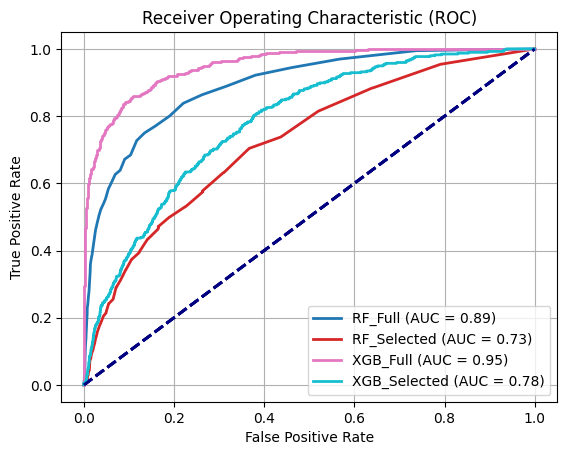
\includegraphics[width=1\textwidth]{figures/ROC.png}
    \caption{ROC Curves Comparison for All Four Models}
    \label{fig:roc_curves}
\end{figure}

\textbf{Model-Specific ROC Performance:}

\begin{itemize}
    \item \textbf{XGB\_Full (AUC = 0.95):} Exhibits exceptional discriminative ability with the curve positioned closest to the top-left corner, indicating optimal sensitivity-specificity balance across all threshold values.
    
    \item \textbf{RF\_Full (AUC = 0.89):} Demonstrates strong performance but with noticeable deviation from the optimal curve, particularly in the high-sensitivity region crucial for bankruptcy detection.
    
    \item \textbf{XGB\_Selected (AUC = 0.78):} Shows moderate discriminative ability with significant performance degradation compared to the full feature variant, highlighting the importance of comprehensive feature sets.
    
    \item \textbf{RF\_Selected (AUC = 0.73):} Exhibits the weakest performance with substantial deviation from optimal classification, indicating limitations in both algorithmic approach and feature representation.
\end{itemize}

\section*{Feature Importance Analysis}

Feature importance analysis revealed key financial indicators driving bankruptcy predictions.
Both Random Forest and XGBoost models have option to calculate feature importance.
The feature importance is calculated by the mean decrease in impurity (MDI) for Random Forest and gain for XGBoost.
The top 10 most important features for Random Forest and XGBoost Full and Selected models are shown in Figure \ref{fig:feature_importance_RF} and Figure \ref{fig:feature_importance_XGB} respectively.

\begin{figure}[H]
    \centering
    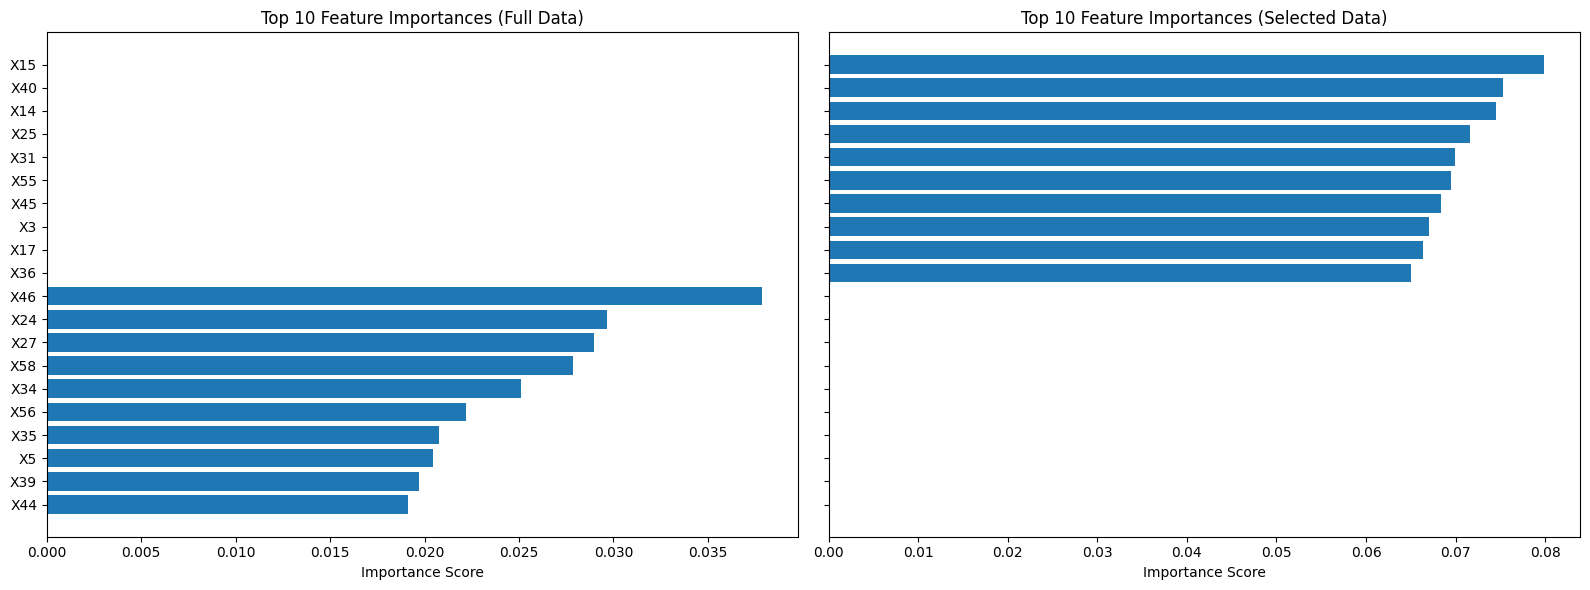
\includegraphics[width=1\textwidth]{figures/Top10_RF.png}
    \caption{Feature Importance Analysis for Random Forest Models}
    \label{fig:feature_importance_RF}
\end{figure}

\begin{figure}[H]
    \centering
    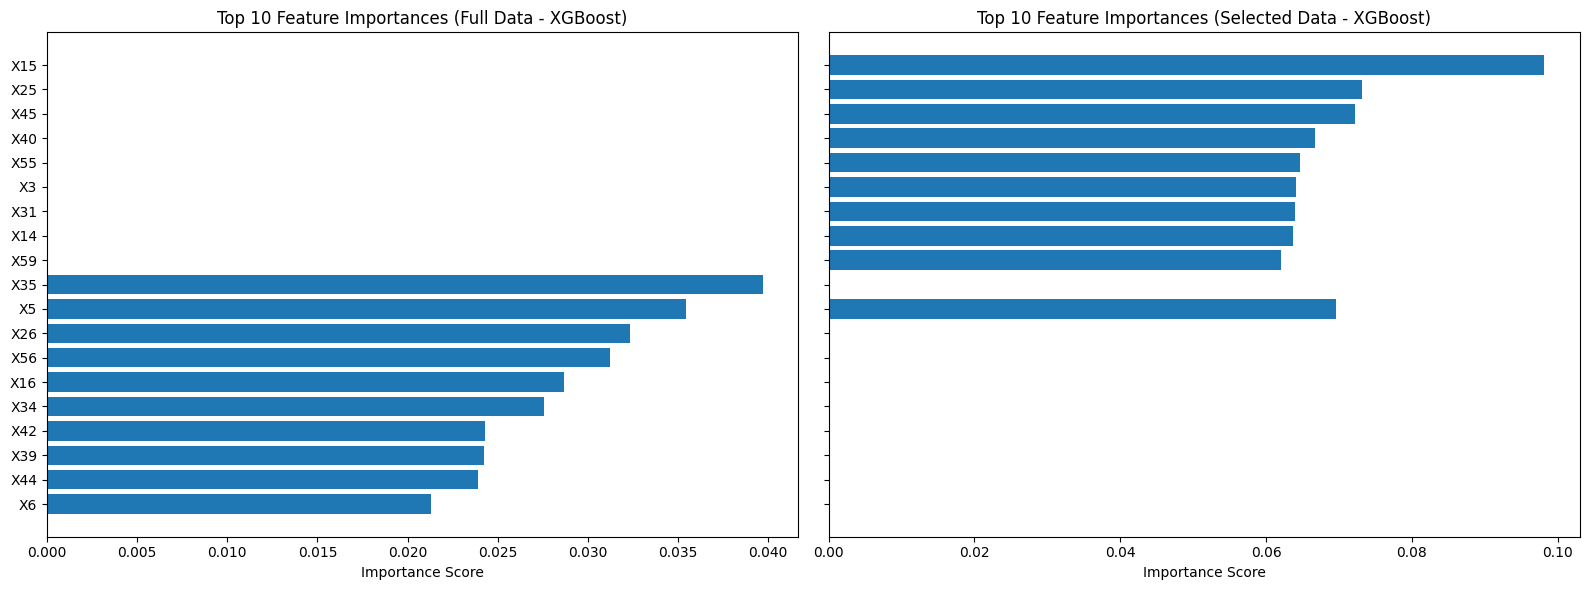
\includegraphics[width=1\textwidth]{figures/Top10_XGB.png}
    \caption{Feature Importance Analysis for XGBoost Models}
    \label{fig:feature_importance_XGB}
\end{figure}

From the feature importance analysis, we can see that the there exists a significant difference between the top 10 most important features for Random Forest and XGBoost models for both full and selected feature models. The reason is that for Selected features we already removed the highly correlated features, which might be in the top features from Full model.
Among 10 important features, 5 features are the common for both Random Forest and XGBoost models with Full data, which are X35, X5, X56, X39,X44. This might be explained by the fact that the Random Forest and XGBoost models are different in the way they calculate feature importance.
For Selected data, there are more common features are X15, X40, X14, X25, X31, X55, X45, X3.

\textbf{Top 5 common Important Features (XGB\_Full and RF\_Full):}
\begin{enumerate}
    \item X35: Profit on sales / total assets
    \item X5: [(cash + short-term securities + receivables - short-term liabilities) / (operating expenses - depreciation)]*365
    \item X56: (sales - cost of products sold) / sales
    \item X39: Profit on sales / sales
    \item X44: (receivables * 365) / sales
\end{enumerate}

All models underwent rigorous 5-fold cross-validation during hyperparameter optimization, ensuring robust performance estimates and reducing overfitting risks. The cross-validation results demonstrated consistent performance across folds, validating the reliability of the modeling approaches.

Early stopping mechanisms were implemented in XGBoost training to prevent overfitting and optimize model complexity. The training process monitored both training and validation AUC scores, terminating when validation performance plateaued to ensure optimal generalization.

Training times varied significantly across models, with Random Forest models generally requiring longer training periods due to the larger ensemble sizes (100 trees vs. optimized boosting rounds in XGBoost). The selected feature models demonstrated reduced computational requirements while maintaining reasonable performance levels, highlighting the trade-off between feature complexity and computational efficiency. 